\chapter{Астрометрический подход к поиску двойных систем} \label{ch:ch1}

\section{Исторический опыт астрометрического исследования быстрых звезд} \label{sec:ch1/sec1}

Развитие методов фотографической астрометрии на рубеже XIX--XX веков позволило начать массовое определение собственных движений звезд, не входящих в каталоги, построенные на основе меридианных наблюдений. Следствием этого стало открытие в 1916 году Эдвардом Барнардом звезды, с самым большим собственным движением \todo{(Barnard, E. E. (1916))}. Сравнительно быстрое перемещение звезды Барнарда на фоне соседей ($\mu$~=~10.358~$''$/yr) закрепило за ней название \glqq летящей\grqq . Звезда Барнарда не является ближайшей к Солнцу, однако ожидаемо входит в наиболее тесное с нами звёздное соседство. Расстояние до \glqq летящей\grqq  звезды чуть более 1.8~пк, и она является четвёртой известной звездой по мере удаления от Солнца, уступая в близости только системе звёзд Альфа Центравра. Однако, помимо выдающегося собственного движения, она имеет и значительную величину лучевой скорости, при этом приближаясь к Солнцу (\(\textup{М}_r\)~>~110 км/сек), и по оценкам может обогнать ближайшую к нам систему звёзд примерно к 11800 году. Стоит также отметить, что звезда Барнарда является красным карликом "--- представителем одной из наиболее многочисленных групп ближайшего околосолнечного населения Галактики. 

Значительные величины собственных движений звезд дают простор для приложения астрометрических исследований в поиске двойных и кратных объектов. Здесь на самом деле речь идет о весьма разнообразных методах. Наиболее старый заключается в попытке обнаружить орбитальное движение для хорошо разрешаемых звездных пар. Эта задача вышла на передний план развития наблюдательной астрономии в конце XVIII века. В 1803 году в мемуарах Гершеля было впервые надежно показано наличие орбитального движения. Этот метод, в основном, касается широких пар с относительно большими периодами обращения (сотни и тысячи лет). Если иметь ввиду солнечную окрестность, то в ее пределах обнаружены десятки двойных систем именно таким способом. От 61-ой Лебедя до современных наблюдений \todo{(например, проект RECONS - http://www.recons.org/)}. 

Массовые и сравнительно точные обзоры собственных движений звезд сразу позволили выявить пары, компоненты которых характеризуются \glqq общим\grqq\ собственным движением. Действительно, для широких пар  скорость движения относительно Солнца заметно больше скорости их взаимного орбитального движения. Поэтому малые различия собственного движения между компонентами оптически двойной с большой вероятностью означают физичность пары. Если к этому добавляется еще и приблизительное равенство лучевых скоростей, тогда вопрос об обнаружении двойной системы можно считать практически решенным.

Реализация миссии Hipparcos больше четверти века назад, и появление первых релизов миссии Gaia повысили интенсивность подобных поисков \todo{(например, Knapp \& Nanson, (2018))}. Выявлено множество широких пар двойных звезд на основе совместного анализа всей астрометрической информации: параллаксов, собственных движений и лучевых скоростей \todo{(например, Kervella et al., (2019))}.

Отдельного рассмотрения заслуживает метод обнаружения так называемых астрометрических двойных звезд (или звезд с невидимыми спутниками). Речь идет о том, что для неразрешаемой при обычных наблюдениях двойной звезды может иметь место значимое различие положений фотоцентра и центра масс. В этом случае наблюдаемое движение звезды становится волнообразным. Наиболее яркий пример - детектирование Фридрихом Бесселем невидимых спутников Сириуса и Проциона. В его работе были проанализированы движения ярчайших звезд неба, используя данные разных обсерваторий за несколько десятилетий. К 1844 году после многолетних наблюдений Проциона и Сириуса Бессель опубликовал вычисления, которые говорили о том, что движения этих звезд имеют заметные периодические отклонения от своих средних долгопериодических трендов, то есть не отличаются прямолинейностью. Наблюдаемые фотоцентры описывали волнообразные линии, что говорило о наличии невидимых спутников у обеих звезд. Позднее эти выводы были подтверждены двумя американскими астрономами. В 1862 году Алван Кларк и в 1896 году Джон Шеберле сумели пронаблюдать ранее невидимые компоненты систем Сириуса (спектральный класс первой компоненты - A1) и Проциона (класс F) соответственно. Эти спутники, характеризуются низкой светимостью и оказались белыми карликами. Данный подход нашел свое развитие и в эпоху космической астрометрии и оказался приемлемым для сравнительно ярких звезд с хорошей историей астрометрических наблюдений. Примером такого исследования является работа \todo{Гончарова и Кияевой (2002)}.

\section{Анализ собственных движений, определенных на разных временных интервалах. Метод Вилена} \label{sec:ch1/sec2}
Как было показано в предыдущем разделе, выявление нелинейности движения по небесной сфере требует хорошей наблюдательной истории - нескольких десятков положений, полученных в разные эпохи. Свойства движений компонент двойных систем определили возможность массового поиска неразрешенных звездных пар без необходимости иметь большое количество точных положений. Достаточно иметь оценки собственных движений, полученные на разных временных интервалах. При достаточно высокой точности определения координат может быть достаточно всего трех положений.

 Собственные движения определены для огромного количества звезд в ходе реализации разнообразных наблюдательных проектов. Это дало возможность массового обнаружения звезд, которые имеют явные признаки двойственности. В 1999 году был представлен метод поиска неразрешаемых двойных систем, основанный на статистическом анализе наблюдаемых изменений собственных движений звезд \todo{(Wielen et al., 1999)}. В работе исследовались ярчайшие звезды, полученные в ходе миссии Hipparcos. Высокая точность определения положений звезд с помощью  астрометрического спутника (порядка 1 mas) раскрыла новые пути поиска и исследования двойных систем \todo{(ESA, 1997)}. Основная идея метода Вилена проиллюстрирована на рисунке~\ref{fig:widea}. Для физической одиночной звезды собственное движение, измеренное в течение короткого промежутка времени, в пределах точности измерений должно совпадать с собственными движением, полученным из очень длинного временного интервала. И в общем случае такого совпадения не будет наблюдаться для неразрешаемой двойной звезды. Из-за гравитационного влияния более слабой компоненты, движение двойной звезды будет волнообразным, что может определить значительное отличие мгновенно измеренного собственного движения от долгосрочного (в идеале - движение барицентра системы). Такую разницу в работе назвали \glqq космической ошибкой\grqq\ и обозначили как $\Delta\mu$. При значительном преобладании космической ошибки по сравнению с ошибкой измерения объект относился к кандидатам в двойные и обозначался как \glqq Дельта-мю двойная\grqq\ (\glqq $\Delta\mu$--binaries\grqq ). Объекты, у которых космическая ошибка была в рамках ошибки наблюдений, были обозначены как \glqq кандидаты в одиночные звезды\grqq\  (\glqq single-star candidate\grqq ), если не было другой информации об их двойственной природе.

\begin{figure}[h]
 \centering
 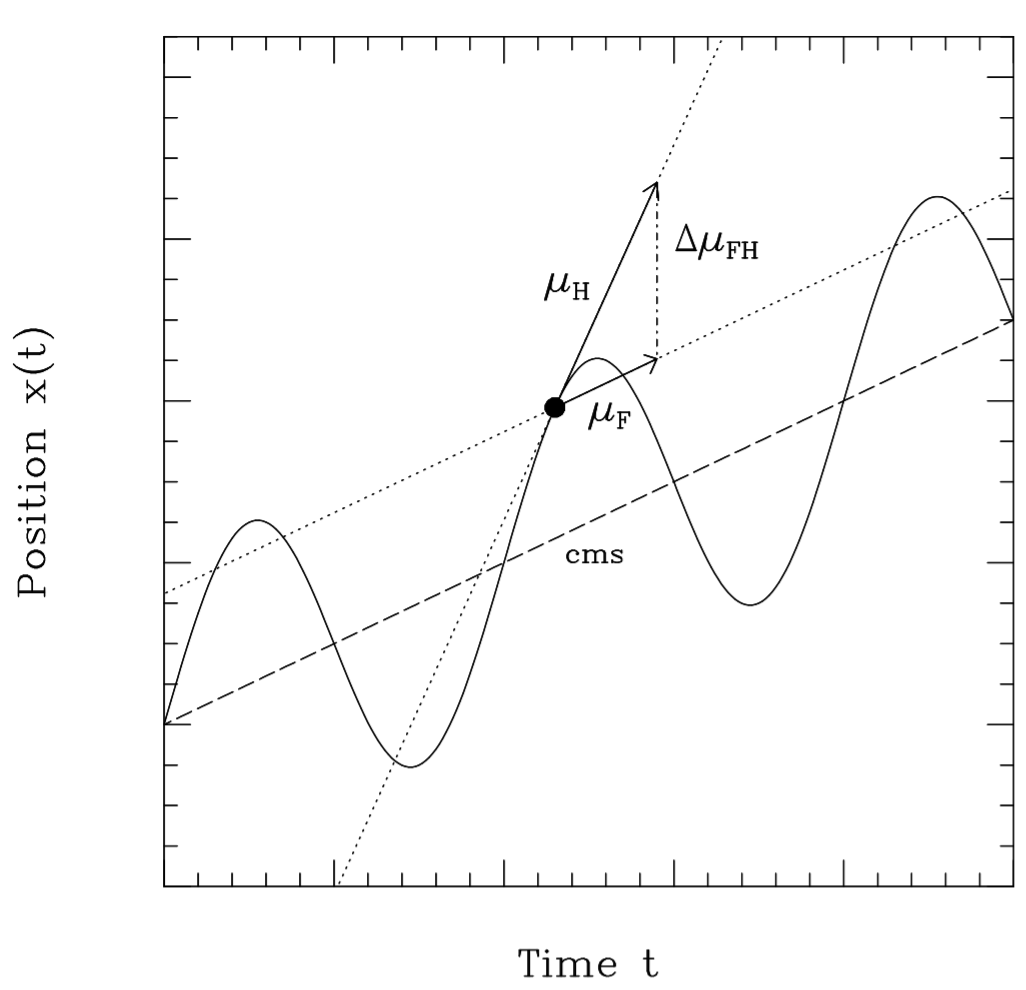
\includegraphics [scale=0.5] {Wielen-idea}
 \caption{Колебания астрометрической двоичной системы, вызванные влиянием орбитального движения, приводит к заметной разнице $\Delta\mu_{FH}$ между мгновенно измеренным собственным движением Hipparcos $\mu_{H}$ и средним собственным движением $\mu_{F}$ фотоцентра. Здесь период обращения двойной системы имеет среднюю длину ($\approx$30 лет), так что собственное движение $\mu_{F}$, полученное из наземных данных (например, из FK5), по существу равно собственному движению барицентра (cms) двойной звезды. Взято из \todo{Wielen et al. (1999, Рис. 1)}.}
 \label{fig:widea}
\end{figure}

В качестве квази-мгновенных были взяты высокоточные собственные движения HIPPARCOS \todo{(ESA 1997)}, $\mu_{H}$, полученные за период около 3 лет в 1991 году. В качестве квази--средних "--- собственные движения, полученные несколькими способами. 

В первую очередь для вычисления квазисредних (\glqq долгосрочных\grqq ) собственных движений использовался каталог FK5 \todo{(Fricke et al., 1988, 19991)}. Из него были извлечены собственные движения ($\mu_F$), а также положения звезд для вычисления новых собственных движений совместно с положениями HIPPARCOS ($\mu_{0F}$), временная база которых составила в среднем 40 лет. Ошибки вычисленных собственных движений оказались значительно меньше, чем указанные в FK5. Их точность обеспечили относительно маленькие ошибки положений FK5 и значительная разница эпох FK5 и HIPPARCOS. Таким образом были получены по 3 разности собственных движений для каждой из координат $\delta$  и $\alpha ^*$~=~$\alpha\,\cos\delta$. Стоит отметить, что положения, взятые из FK5, для одной звезды могли не совпадать по эпохе для разных координат. Это несколько усложнило физическую интерпретацию результатов исследования, однако исключило корреляции в собственных движениях по разным координатам.

Помимо каталога FK5 в исследовании был использован каталог GC \todo{(Boss et al., 1937)}. Хотя количество объектов GC (33\,342) сильно больше, чем в FK5 (4\,652), низкая точность собственных движений этого каталога не позволила использовать собственные движения, опубликованные в GC. Однако огромная разница эпох наблюдения с HIPPARCOS позволила получить новые собственные движения ($\mu_{0}$(GC)). Также стоит отметить, что большое пересечение выборки FK5 и GC обеспечило проверку согласованности данных.

Для вычисления ошибок получаемых $\Delta\mu$ авторы использовали ошибки собственных движений из каталога HIPPARCOS, а так же комбинацию индивидуальных ошибок собственных движений наземных каталогов со значениями систематических ошибок редукции каталогов в систему HIPPARCOS.

В ходе исследования статистических особенностей данных авторы учли тот факт, что собственные движения HIPPARCOS по двум координатам коррелируют. По данным в каталоге коэффициентам корреляции была построена ковариация, которая позволила скорректировать (повернуть на угол $\psi$) оси собственных движений таким образом, чтобы они соответствовали осям эллипсоида ошибок (см. рисунок~\ref{fig:werr}). Вдоль новых осей авторами были определены формулы дисперсий ожидаемого гауссовского распределения ошибок.

Для оценки статистической значимости $\Delta\mu$ был выведен тестовый  параметр оценки $F_{0H}$:

\begin{equation}
  \label{eq:WiF}
  F^{2}_{0H} =(\frac{\Delta\mu_{0H,\psi}}{\epsilon_{\Delta\mu_{0H,\psi}}})^{2}+(\frac{\Delta\mu_{0H,\bar{\psi}}}{\epsilon_{\Delta\mu_{0H,\bar{\psi}}}})^{2}
\end{equation}

Если звезда не является двойной, то ожидается, что некоррелированные переменные $\Delta\mu_{0H,\psi}$ и  $\Delta\mu_{0H,\bar{\psi}}$ будут следовать нормальным распределениям со средним нулем и дисперсиями, определенными авторами ранее. В этом случае вероятность $W(F)$ случайно найти значение $F_{0H}$, равное или превышающее наблюдаемое значение, определялось уравнением:

\begin{equation}
  \label{eq:WiW}
  W(F) = e^{-F^2_{0H}/2}
\end{equation}

Плотность вероятности $w(F)dF$, показывающая вероятность нахождения $F_{0H}$ между $F$ и $F+dF$ определяется как:

\begin{equation}
  \label{eq:Wiww}
  w(F) = -\frac{dW(F)}{dF} = F_{0H}\,e^{-F^2_{0H}/2}
\end{equation}

Характер этих функций (см. рисунок~\ref{fig:wWw}) дал основание полагать, что высокое наблюдаемое значение $F_{0H}$ является значимым показателем двойственной природы исследуемого объекта. В качестве минимального значения $F_0H$, при котором звезду относили к $\Delta\mu$--двойным, авторы определили как $F_{lim,b}=3.44$, который дает $W(3.44)=0.0027$, что удовлетворяет критерию 3$\sigma$. Вторым пограничным значением $F_0H$, ниже которого звезда считалась кандидатом в одиночную стало $F_{lim,s}=2.49$, что соответствует критерию 2$\sigma$ ($W(2.49)=0.0456$).

 \begin{figure}[h]
 \centering
 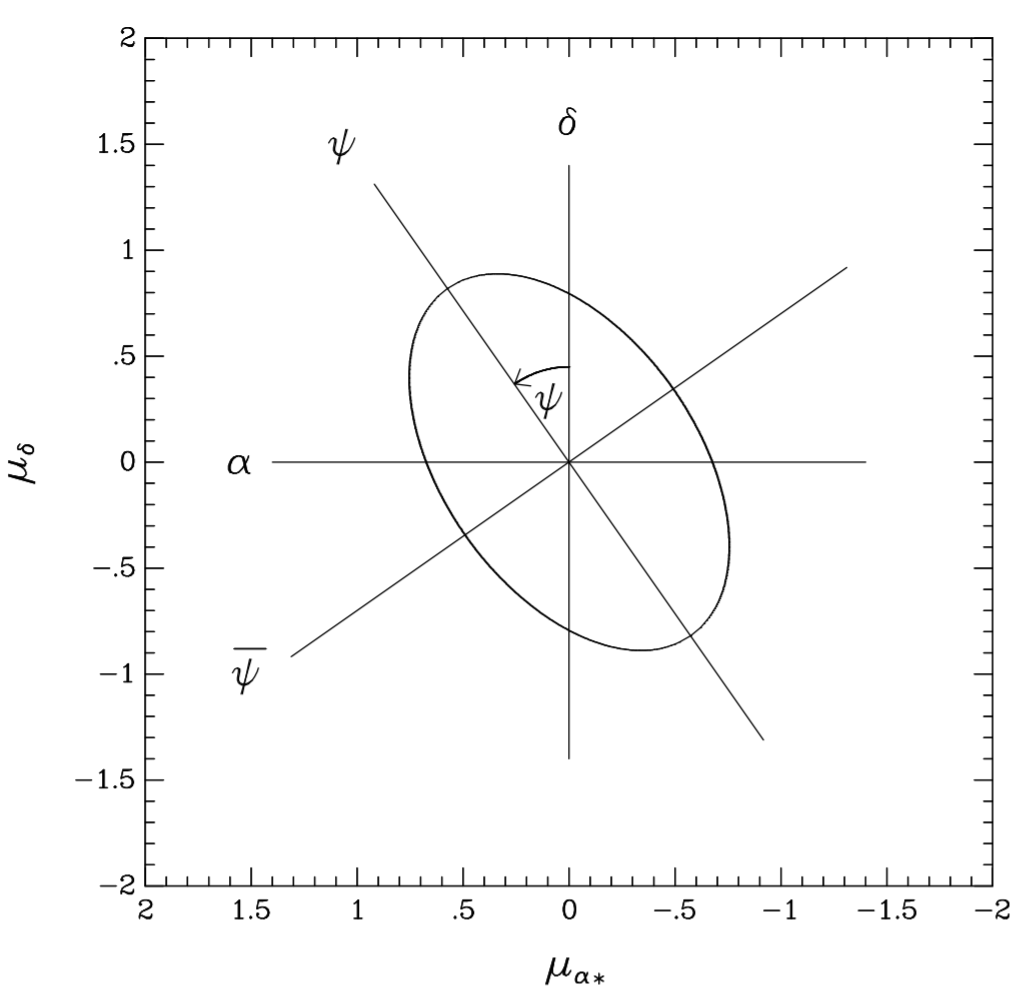
\includegraphics [scale=0.5] {Wielen-err}
 \caption{Эллипсоид ошибок измерений $\Delta\mu$, наклонен относительно экваториальной системы ($\delta$, $\alpha^*$) на угол $\psi$. Большая ось эллипсоида ошибок указывает в направлении $\psi$, малая ось "--- в направлении $\bar{\psi}$.  Взято из \todo{Wielen et al. (1999, Рис. 2)}.}
 \label{fig:werr}
\end{figure}

Тогда как для звезд представленных только в CG есть только одно значение $F_{0}(GC)$, для звезд FK5 в общем случае доступно 3 параметра оценки ($F_{FH}$, $F_{0H}$, $F_{0F}$). Авторы предлагают считать объект $\Delta\mu$--двойным, если хотя бы 1 из величин больше, чем $F_{lim,b}$. Для кандидата в одиночную звезду, все значения должны быть меньше $F_{lim,s}$.

Авторы отмечают, что данный метод имеет ограничения. К примеру, он не применим к двойным звездам, чей период орбитального движения менее 3 лет, а для звезд с очень большими периодами (порядка 1000 лет) метод требует чрезвычайно высокой точности. Однако, он хорошо работает для близких быстрых звезд, чей период составляет десятки лет.  В результате проведенной работы было обнаружено больше тысячи впервые детектированных $\Delta\mu$--двойных звезд, что составило примерно 10\,\% от исследованных.

 \begin{figure}[h]
 \centering
 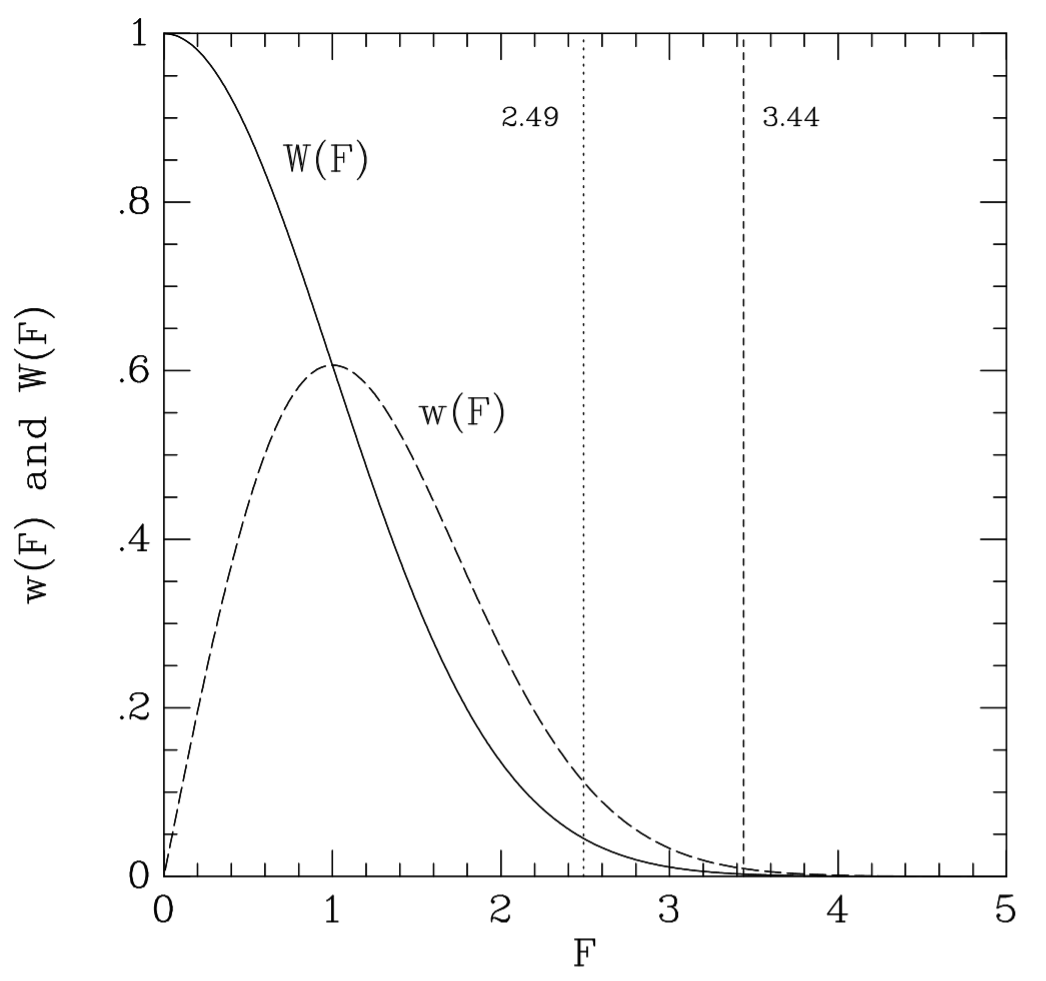
\includegraphics [scale=0.5] {Wielen-Ww}
 \caption{Функция W(F) описывает вероятность случайного нахождения наблюдаемого значения тестового параметра, большего чем F. Функция w(F) является дифференциальной вероятностью. Указаны два критических значения: F~>~3.44 для $\Delta\mu$--двойных и F~<~2.49 для кандидатов в одиночную звезду. Взято из \todo{Wielen et al. (1999, Рис. 3)}.}
 \label{fig:wWw}
\end{figure}

Напомним, что исследования Вилена и его коллег затрагивают яркие звезды из состава FK5 и HIPPARCOS. В основном это объекты в диапазоне от солнцеподобных звезд до звезд ранних спектральных классов главной последовательности и гигантов, распределенные в ближайших 100 пк от Солнца. Объекты нашего исследования "--- звезды--карлики ближайшего окружения Солнца. Но, с некоторыми усовершенствованиями, идея Вилена вполне применима к поиску двойных систем для этого типа объектов. 

\section{Исследования близких карликов в Пулковской обсерватории} \label{sec:ch1/sec3}
В последнее десятилетие в Пулковской обсерватории активно реализуется комплексная программа изучения звезд с большими собственными движениями, включающая определение тригонометрических параллаксов  \todo{(Хруцкая и др., 2010, Ховричев и др., 2013)}, уточнение собственных движений, анализ кинематики \todo{(Хруцкая и др. 2009)}. В том числе реализуется изложенный выше подход к детектированию двойных карликов. Метод Вилена был адаптирован для исследования звезд низкой светимости с большими значениями собственного движения. Наиболее подробное изложение адаптации и реализации метода Вилена в пулковской программе будет изложено в главе 3. Первая попытка применения данного подхода \todo{(Хруцкая и др, 2011)} была предпринята на материале звезд-карликов, расположенных в зенитной зоне Пулковской обсерватории (от $30^{o}$ до $70^{o}$ по склонению). Наблюдения были проведены с помощью Нормального астрографа. В наблюдательную программу вошли 1123 звезды с большими собственными движениями ($\mu$~>~300~mas/yr). Следующая работа \todo{(Ховричев, Куликова, 2015)} содержит исследования практически всех быстрых звезд, относимых к категории близких карликов и доступных для наблюдений в Пулкове. Для дальнейшего анализа были вычислены собственные движения, однако в отличие от первой реализации положения звезд брались не из каталогов, а были получены методами прямой редукции с кадра на кадр, это позволило избежать систематических ошибок каталогов, однако встал вопрос о реализации способа вычисления пиксельных координат. На первом этапе использовался МНК, однако в дальнейшей хорошо зарекомендовал себя адаптированный для исследования изображений звезд метод shapelet-формализма, описанию которого посвящена следующая глава. Этот метод дал возможность осуществить выявление двойных звезд на основе особенностей их изображений, о чем подробнее сказано в главе 4.